\documentclass[withoutpreface,bwprint]{cumcmthesis}
% \usepackage{subfigure}
\title{基于SEIR改进模型的疫情应对措施分析}

\begin{document}
\maketitle

\section{项目背景}
近年来,人类社会面临着严重的传染病威胁。非典型性肺炎(SARS)、高致病性禽流感H5N1、甲型流感H1N1以及新型冠状病毒肺炎(COVID-19)等传染病的爆发给人们的生命健康和社会生活带来了巨大影响。因此,如何有效遏制传染病的爆发并缓解其流行成为当今社会面临的紧迫问题。

从系统科学的角度来看,传染病的流行是一个复杂的扩散过程,发生在人群中。对这一过程进行建模有助于理解传染病的流行机理,并认识其中的内在规律。通过建立合理的模型,可以深入研究传染病的传播途径、传播速度、传染源的特征以及人群的行为模式等因素,从而为制定干预措施提供理论依据。

建立传染病模型可以通过数学方法和计算机模拟来实现。数学方法可以用来表达传染病的传播动力学,如人群的感染率、康复率和死亡率等,从而预测传染病的发展趋势。计算机模拟则可以模拟人群的行为和交流,以及传染病在人群中的传播过程,从而评估不同干预措施的效果。

基于传染病模型的研究可以为公共卫生政策制定提供科学依据。通过模拟不同干预措施的效果,可以评估其对传染病传播的抑制程度,并为政府和卫生部门提供决策支持。
\section{研究内容}
\subsection{模型选择}
目前,对传染病流行过程的建模已经发展出了多种范式,概括来说,可以分为:单一群体方法、
复合群体方法和微观个体方法。主要有三种方法 第一种是单一群体方法:将人群看作一个整,流
行过程表现在易感者,感染者等各类人员集计量的变化;第二种是复合群体方法:考虑人群在空间上的异质
性,将人群划分为多个子群体,各子群体之间因人员流动而藕合,形成复杂动态系统;第三种
是微观个体方法:建模出发点是人群中的个体,个体有各自的属性和行为规则,个体之间形成接触网络,感染
者和易感者的接触导致易感个体状态的变化,形成网络上的传播动力学过程。三种建模方法的基本思想如\cref{fig:1}。
\begin{figure}[H]
    \centering
    \begin{minipage}[c]{0.3\textwidth}
        \centering
        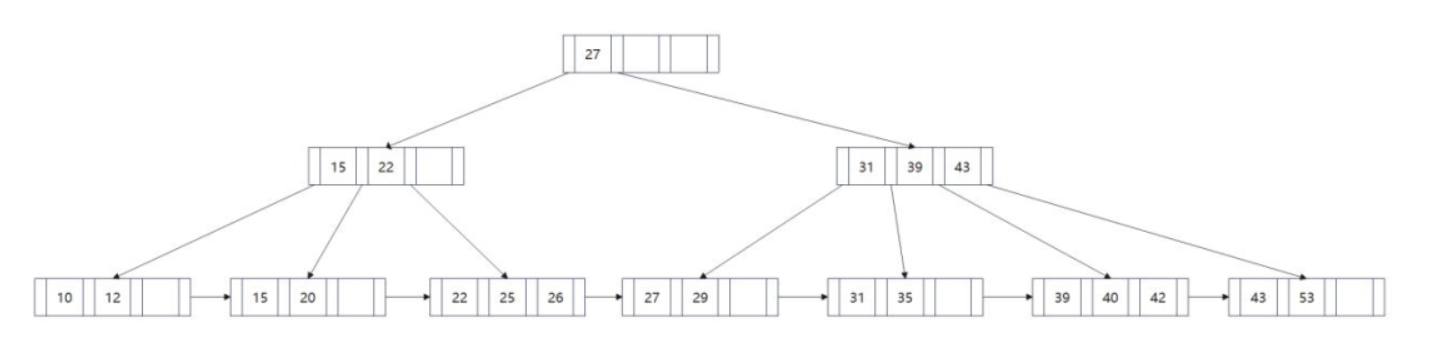
\includegraphics[width=0.95\textwidth]{2}
        \subcaption{单一群体方法}
        \label{fig:1.1}
    \end{minipage}
    \begin{minipage}[c]{0.3\textwidth}
        \centering
        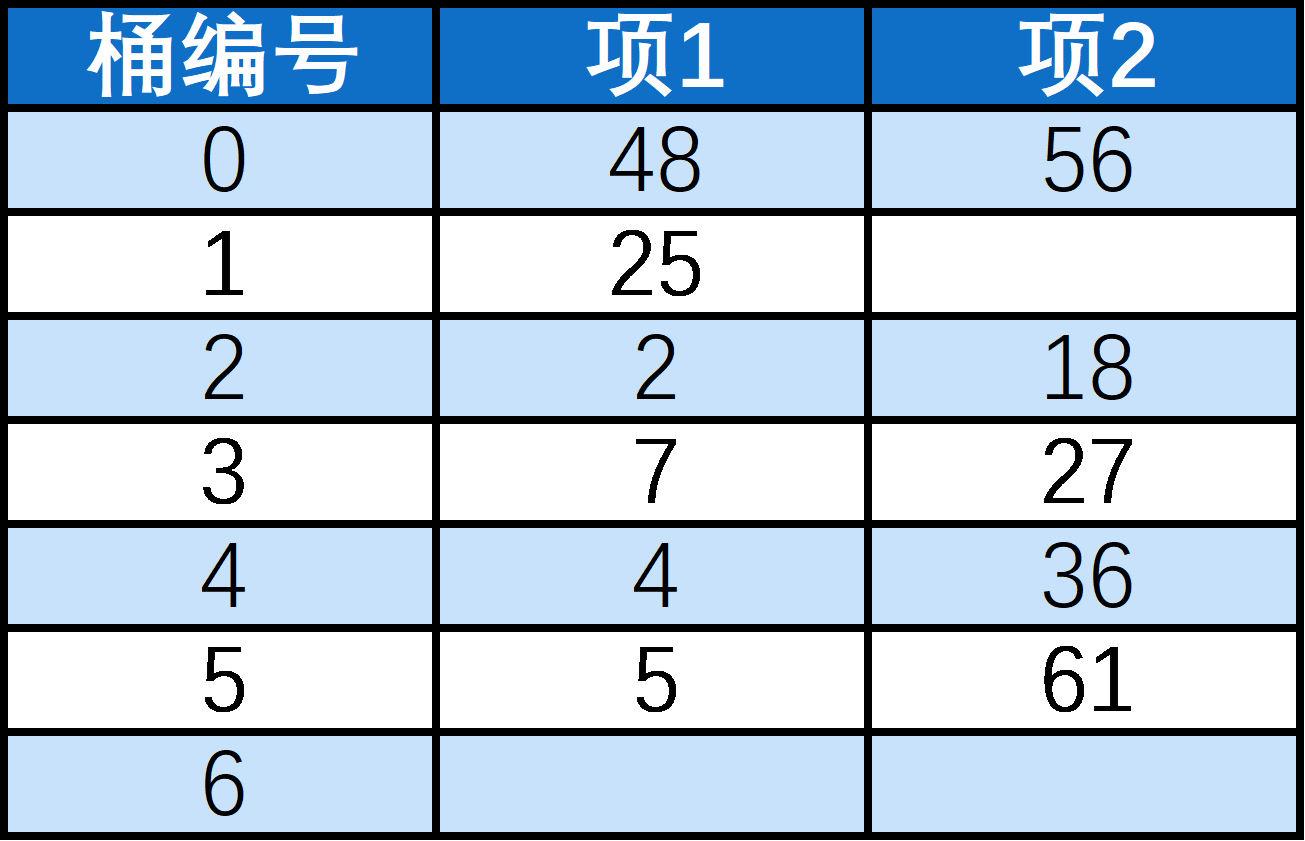
\includegraphics[width=0.95\textwidth]{3}
        \subcaption{复合群体方法}
        \label{fig:1.2}
    \end{minipage}
    \begin{minipage}[c]{0.3\textwidth}
        \centering
        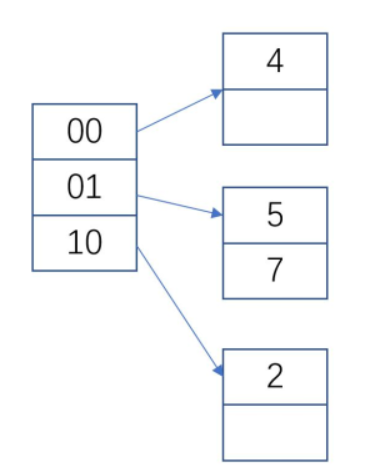
\includegraphics[width=0.95\textwidth]{1}
        \subcaption{微观个体方法}
        \label{fig:1.3}
    \end{minipage}
    \caption{传染病传播三种建模方法}
    \label{fig:1}
\end{figure}

\par
在这里,选择单一群体方法中的SEIR模型作为基础模型,如\cref{fig:2},在基于SEIR模型的改进模型上进行分析。
\begin{figure}[H]
    \centering
    \includegraphics[width=0.95\textwidth]{SEIR_model}
    \caption{SEIR模型}
    \label{fig:2}
\end{figure}

\subsection{模型改进}
\subsubsection{模型拓扑结构的改进}
传统的SEIR模型将人群分为易感人群、潜伏期人群、感染人群和康复人群。人群划分较为粗糙,
与现实情况拟合结果较差。

而在应对2019年底开始的新型冠状病毒肺炎疫情中,隔离措施被实践证明是一种有效的减缓传染病流行的措施。
将隔离措施纳入考虑,进一步将易感人群、潜伏期人群和感染人群进一步划分为普通易感人群$S$、被隔离的易感人群$S_q$、
普通潜伏期人群$E$、被隔离的潜伏期人群$E_q$、未被收治的感染人群$I$和被隔离收治的感染人群$I_q$。同时考虑疾病导致的死亡,增加因病死亡人群$D$。
新的模型拓扑结构如\cref{fig:3}。

\begin{figure}[H]
    \centering
    \includegraphics[width=0.95\textwidth]{SEIRQD_model}
    \caption{改进模型的拓扑结构}
    \label{fig:3}
\end{figure}


\subsubsection{模型参数的改进}
在传统的SEIR模型中,各个人群之间的转移参数各自独立,无法挖掘出各个参数之间的关系以及各个参数的实际指导意义。
因此,考虑到改进模型的人群划分,将参数重新设置,增强其关联性和实际意义。新设置的参数如\cref{fig:4}。

\begin{figure}[H]
    \centering
    \includegraphics[width=0.95\textwidth]{SEIRQD}
    \caption{改进模型的参数设置}
    \label{fig:4}
\end{figure}
\par
各个参数含义如\cref{tb:1}。
\begin{table}[H]
    \caption{参数含义}\label{tb:1}
    \resizebox{\textwidth}{!}{
        \begin{tabular}{cc}
            \toprule[1.5pt]
            名称         & 含义                                       \\
            \midrule[1pt]
            $\rho$     & 易感人群被追踪到的概率,可以视为对普通群众的隔离强度               \\
            $\omega$   & 被隔离的易感人群接触隔离的速度,即隔离时长的倒数                 \\
            $\beta$    & 一天中易感人群和潜伏期人群或感染人群的有效接触次数,可视为普通群众的防范意识强弱 \\
            $\varphi$  & 传染病传染强度                                  \\
            $\epsilon$ & 潜伏期人群相较于染病人群的感染能力大小                      \\
            $\alpha$   & 潜伏期人群转变为染病人群的速度,即潜伏期的倒数                  \\
            $\theta$   & 收治感染人群的速度,可视为医疗资源的倾斜程度                   \\
            $\gamma_I$ & 未被收治的感染人群康复速度,可视为人体自愈能力大小                \\
            $\gamma_q$ & 被收治的感染人群康复速度,可视为药物研发重视程度                 \\
            $d$        & 未被收治的感染人群死亡速度,为1-$\gamma_I$              \\
            $d_q$      & 被收治的感染人群死亡速度,为1-$\gamma_q$               \\
            \bottomrule[1.5pt]
        \end{tabular}
    }

\end{table}



\subsection{模型建立}

改进后的模型如\cref{fig:3},其对应的微分方程组如\cref{eq:1}。
\begin{equation}
    \begin{cases}
        \frac{dS}{dt}=-(1-\rho)\varphi\beta(I+\epsilon E)S-\rho\varphi\beta(I+\epsilon E)S-\rho(1-\varphi)\beta(I+\epsilon E)S+\omega S_q \\
        \frac{dE}{dt}=(1-\rho)\varphi\beta(I+\epsilon E)S-\alpha E                                                                        \\
        \frac{dI}{dt}=\alpha E-\gamma_II-d_II-\theta I                                                                                    \\
        \frac{dR}{dt}=\gamma_II+\gamma_qI_q                                                                                               \\
        \frac{dS_q}{dt}=\rho(1-\varphi)\beta(I+\epsilon E)S-\omega S_q                                                                    \\
        \frac{dE_q}{dt}=\rho\varphi\beta(I+\epsilon E)S-\alpha E_q                                                                        \\
        \frac{dI_q}{dt}=\alpha E_q-\gamma_qI_q-d_qI_q+\theta I                                                                            \\
        \frac{dD}{dt}=dI+d_qI_q
    \end{cases}
    \label{eq:1}
\end{equation}

在模型中,参数$\rho$、$\beta$、$\theta$、$\gamma_q$、$\omega$是可人为控制的,之后对这几个参数进行分析。
同时考虑到不同烈度的传染病和传染病流行的不同时期对于应对策略的选择均会产生影响,因此,将传染病分为低烈度,中烈度,高烈度三种,研究
在流行前期,中期,后期上述参数对于传染病继续流行50天后的死亡率的影响。
不同情况下模型初始参数设置如\cref{fig:5}。

\begin{figure}[H]
    \centering
    \includegraphics[width=0.95\textwidth]{args_in_cases}
    \caption{不同情况下模型参数设置}
    \label{fig:5}
\end{figure}


\section{结果分析}
在这里,分别对上一节中设置的9种不同情况分别进行分析,其中参数$\omega$这里用隔离天数$T$代替。待研究参数默认值以及其对应浮动范围如\cref{tb:2}
\begin{table}[H]
    \caption{参数含义}\label{tb:2}
    \centering
    \begin{tabular}{ccc}
        \toprule[1.5pt]
        参数         & 默认值   & 取值范围        \\
        \midrule[1pt]
        $\rho$     & $0.5$ & $0.1-0.9$   \\
        $T$        & $7$   & $1-14$(取整数) \\
        $\beta$    & $5$   & $0.5-10$    \\
        $\theta$   & $0.5$ & $0.1-0.9$   \\
        $\gamma_q$ & $0.5$ & $0.1-0.9$   \\
        \bottomrule[1.5pt]
    \end{tabular}
\end{table}

\subsection{高烈度前期}

对于高烈度传染病传播前期各参数对继续流行50天后的死亡率影响如\cref{fig:6}
\begin{figure}[H]
    \centering
    \begin{minipage}[c]{0.3\textwidth}
        \centering
        \includegraphics[width=0.95\textwidth]{images/1/rho}
        \subcaption{$\rho$}
    \end{minipage}
    \begin{minipage}[c]{0.3\textwidth}
        \centering
        \includegraphics[width=0.95\textwidth]{images/1/T}
        \subcaption{$T$}
    \end{minipage}
    \begin{minipage}[c]{0.3\textwidth}
        \centering
        \includegraphics[width=0.95\textwidth]{images/1/beta}
        \subcaption{$\beta$}
    \end{minipage}

    \begin{minipage}[c]{0.3\textwidth}
        \centering
        \includegraphics[width=0.95\textwidth]{images/1/theta}
        \subcaption{$\theta$}
    \end{minipage}
    \begin{minipage}[c]{0.3\textwidth}
        \centering
        \includegraphics[width=0.95\textwidth]{images/1/gamma_q}
        \subcaption{$\gamma_q$}
    \end{minipage}
    \caption{高烈度前期各参数对死亡率影响}
    \label{fig:6}

\end{figure}

\subsection{高烈度中期}

对于高烈度传染病传播中期各参数对继续流行50天后的死亡率影响如\cref{fig:7}
\begin{figure}[H]
    \centering
    \begin{minipage}[c]{0.3\textwidth}
        \centering
        \includegraphics[width=0.95\textwidth]{images/2/rho}
        \subcaption{$\rho$}
    \end{minipage}
    \begin{minipage}[c]{0.3\textwidth}
        \centering
        \includegraphics[width=0.95\textwidth]{images/2/T}
        \subcaption{$T$}
    \end{minipage}
    \begin{minipage}[c]{0.3\textwidth}
        \centering
        \includegraphics[width=0.95\textwidth]{images/2/beta}
        \subcaption{$\beta$}
    \end{minipage}

    \begin{minipage}[c]{0.3\textwidth}
        \centering
        \includegraphics[width=0.95\textwidth]{images/2/theta}
        \subcaption{$\theta$}
    \end{minipage}
    \begin{minipage}[c]{0.3\textwidth}
        \centering
        \includegraphics[width=0.95\textwidth]{images/2/gamma_q}
        \subcaption{$\gamma_q$}
    \end{minipage}
    \caption{高烈度中期各参数对死亡率影响}
    \label{fig:7}

\end{figure}

\subsection{高烈度后期}
对于高烈度传染病传播前期各参数对继续流行50天后的死亡率影响如\cref{fig:8}
\begin{figure}[H]
    \centering
    \begin{minipage}[c]{0.3\textwidth}
        \centering
        \includegraphics[width=0.95\textwidth]{images/3/rho}
        \subcaption{$\rho$}
    \end{minipage}
    \begin{minipage}[c]{0.3\textwidth}
        \centering
        \includegraphics[width=0.95\textwidth]{images/3/T}
        \subcaption{$T$}
    \end{minipage}
    \begin{minipage}[c]{0.3\textwidth}
        \centering
        \includegraphics[width=0.95\textwidth]{images/3/beta}
        \subcaption{$\beta$}
    \end{minipage}

    \begin{minipage}[c]{0.3\textwidth}
        \centering
        \includegraphics[width=0.95\textwidth]{images/3/theta}
        \subcaption{$\theta$}
    \end{minipage}
    \begin{minipage}[c]{0.3\textwidth}
        \centering
        \includegraphics[width=0.95\textwidth]{images/3/gamma_q}
        \subcaption{$\gamma_q$}
    \end{minipage}
    \caption{高烈度后期各参数对死亡率影响}
    \label{fig:8}

\end{figure}

\subsection{中烈度前期}

对于中烈度传染病传播前期各参数对继续流行50天后的死亡率影响如\cref{fig:9}
\begin{figure}[H]
    \centering
    \begin{minipage}[c]{0.3\textwidth}
        \centering
        \includegraphics[width=0.95\textwidth]{images/4/rho}
        \subcaption{$\rho$}
    \end{minipage}
    \begin{minipage}[c]{0.3\textwidth}
        \centering
        \includegraphics[width=0.95\textwidth]{images/4/T}
        \subcaption{$T$}
    \end{minipage}
    \begin{minipage}[c]{0.3\textwidth}
        \centering
        \includegraphics[width=0.95\textwidth]{images/4/beta}
        \subcaption{$\beta$}
    \end{minipage}

    \begin{minipage}[c]{0.3\textwidth}
        \centering
        \includegraphics[width=0.95\textwidth]{images/4/theta}
        \subcaption{$\theta$}
    \end{minipage}
    \begin{minipage}[c]{0.3\textwidth}
        \centering
        \includegraphics[width=0.95\textwidth]{images/4/gamma_q}
        \subcaption{$\gamma_q$}
    \end{minipage}
    \caption{中烈度前期各参数对死亡率影响}
    \label{fig:9}

\end{figure}

\subsection{中烈度中期}

对于中烈度传染病传播中期各参数对继续流行50天后的死亡率影响如\cref{fig:10}
\begin{figure}[H]
    \centering
    \begin{minipage}[c]{0.3\textwidth}
        \centering
        \includegraphics[width=0.95\textwidth]{images/5/rho}
        \subcaption{$\rho$}
    \end{minipage}
    \begin{minipage}[c]{0.3\textwidth}
        \centering
        \includegraphics[width=0.95\textwidth]{images/5/T}
        \subcaption{$T$}
    \end{minipage}
    \begin{minipage}[c]{0.3\textwidth}
        \centering
        \includegraphics[width=0.95\textwidth]{images/5/beta}
        \subcaption{$\beta$}
    \end{minipage}

    \begin{minipage}[c]{0.3\textwidth}
        \centering
        \includegraphics[width=0.95\textwidth]{images/5/theta}
        \subcaption{$\theta$}
    \end{minipage}
    \begin{minipage}[c]{0.3\textwidth}
        \centering
        \includegraphics[width=0.95\textwidth]{images/5/gamma_q}
        \subcaption{$\gamma_q$}
    \end{minipage}
    \caption{中烈度中期各参数对死亡率影响}
    \label{fig:10}

\end{figure}

\subsection{中烈度后期}

对于中烈度传染病传播后期各参数对继续流行50天后的死亡率影响如\cref{fig:11}
\begin{figure}[H]
    \centering
    \begin{minipage}[c]{0.3\textwidth}
        \centering
        \includegraphics[width=0.95\textwidth]{images/6/rho}
        \subcaption{$\rho$}
    \end{minipage}
    \begin{minipage}[c]{0.3\textwidth}
        \centering
        \includegraphics[width=0.95\textwidth]{images/6/T}
        \subcaption{$T$}
    \end{minipage}
    \begin{minipage}[c]{0.3\textwidth}
        \centering
        \includegraphics[width=0.95\textwidth]{images/6/beta}
        \subcaption{$\beta$}
    \end{minipage}

    \begin{minipage}[c]{0.3\textwidth}
        \centering
        \includegraphics[width=0.95\textwidth]{images/6/theta}
        \subcaption{$\theta$}
    \end{minipage}
    \begin{minipage}[c]{0.3\textwidth}
        \centering
        \includegraphics[width=0.95\textwidth]{images/6/gamma_q}
        \subcaption{$\gamma_q$}
    \end{minipage}
    \caption{中烈度后期各参数对死亡率影响}
    \label{fig:11}

\end{figure}

\subsection{低烈度前期}

对于低烈度传染病传播前期各参数对继续流行50天后的死亡率影响如\cref{fig:12}
\begin{figure}[H]
    \centering
    \begin{minipage}[c]{0.3\textwidth}
        \centering
        \includegraphics[width=0.95\textwidth]{images/7/rho}
        \subcaption{$\rho$}
    \end{minipage}
    \begin{minipage}[c]{0.3\textwidth}
        \centering
        \includegraphics[width=0.95\textwidth]{images/7/T}
        \subcaption{$T$}
    \end{minipage}
    \begin{minipage}[c]{0.3\textwidth}
        \centering
        \includegraphics[width=0.95\textwidth]{images/7/beta}
        \subcaption{$\beta$}
    \end{minipage}

    \begin{minipage}[c]{0.3\textwidth}
        \centering
        \includegraphics[width=0.95\textwidth]{images/7/theta}
        \subcaption{$\theta$}
    \end{minipage}
    \begin{minipage}[c]{0.3\textwidth}
        \centering
        \includegraphics[width=0.95\textwidth]{images/7/gamma_q}
        \subcaption{$\gamma_q$}
    \end{minipage}
    \caption{低烈度前期各参数对死亡率影响}
    \label{fig:12}

\end{figure}

\subsection{低烈度中期}

对于低烈度传染病传播中期各参数对继续流行50天后的死亡率影响如\cref{fig:13}
\begin{figure}[H]
    \centering
    \begin{minipage}[c]{0.3\textwidth}
        \centering
        \includegraphics[width=0.95\textwidth]{images/8/rho}
        \subcaption{$\rho$}
    \end{minipage}
    \begin{minipage}[c]{0.3\textwidth}
        \centering
        \includegraphics[width=0.95\textwidth]{images/8/T}
        \subcaption{$T$}
    \end{minipage}
    \begin{minipage}[c]{0.3\textwidth}
        \centering
        \includegraphics[width=0.95\textwidth]{images/8/beta}
        \subcaption{$\beta$}
    \end{minipage}

    \begin{minipage}[c]{0.3\textwidth}
        \centering
        \includegraphics[width=0.95\textwidth]{images/8/theta}
        \subcaption{$\theta$}
    \end{minipage}
    \begin{minipage}[c]{0.3\textwidth}
        \centering
        \includegraphics[width=0.95\textwidth]{images/8/gamma_q}
        \subcaption{$\gamma_q$}
    \end{minipage}
    \caption{低烈度中期各参数对死亡率影响}
    \label{fig:13}

\end{figure}

\subsection{低烈度后期}

对于低烈度传染病传播后期各参数对继续流行50天后的死亡率影响如\cref{fig:14}
\begin{figure}[H]
    \centering
    \begin{minipage}[c]{0.3\textwidth}
        \centering
        \includegraphics[width=0.95\textwidth]{images/9/rho}
        \subcaption{$\rho$}
    \end{minipage}
    \begin{minipage}[c]{0.3\textwidth}
        \centering
        \includegraphics[width=0.95\textwidth]{images/9/T}
        \subcaption{$T$}
    \end{minipage}
    \begin{minipage}[c]{0.3\textwidth}
        \centering
        \includegraphics[width=0.95\textwidth]{images/9/beta}
        \subcaption{$\beta$}
    \end{minipage}

    \begin{minipage}[c]{0.3\textwidth}
        \centering
        \includegraphics[width=0.95\textwidth]{images/9/theta}
        \subcaption{$\theta$}
    \end{minipage}
    \begin{minipage}[c]{0.3\textwidth}
        \centering
        \includegraphics[width=0.95\textwidth]{images/9/gamma_q}
        \subcaption{$\gamma_q$}
    \end{minipage}
    \caption{低烈度后期各参数对死亡率影响}
    \label{fig:14}

\end{figure}


\section{结论}

根据前述研究结果,可以得出结论:针对中低烈度的传染病,及时实施隔离和个人防护措施是一种高效的控制手段,能够有效遏制传染病的传播。
这意味着,当发现有人感染传染病时,将其隔离并采取适当的个人防护措施,如佩戴口罩和勤洗手,可以有效阻断病原体的传播途径,从而降低传染风险。

对于高烈度的传染病,情况稍有不同。在早期传播阶段,同样可以通过隔离和个人防护来有效遏制传播。这意味着,在发现传染病初期的感染者时,
及时隔离他们,并采取适当的个人防护措施,可以有效限制病原体的传播范围,从而控制传染病的蔓延。

然而,对于中期和后期的传播阶段,仅仅依靠隔离和个人防护的措施已经无法有效地控制传染病的传播。这是因为在这个阶段,传染病的传播已经
广泛而迅速,很难通过个别感染者的隔离来阻断传播链。因此,在这个阶段,除了继续坚持隔离和个人防护的措施外,加大有效药物研发力度并及
时对感染者进行救治成为减少死亡率的唯一可行方法。通过提供适当的医疗救治和支持,可以帮助患者恢复健康,减轻病情的严重程度,并降低死亡率。

因此,无论传染病的烈度如何,及时实施隔离和个人防护是控制传染病传播的重要措施。同时,对于高烈度传染病,早期隔离和个人防护可以有效
遏制传播,但在中期和后期传播阶段,救治感染者是关键。此外,还需要根据传染病的严重程度,合理分配医疗资源,尽力挽救生命。这样才能最
大限度地减少传染病带来的损失,并保护公众的健康。
\end{document}